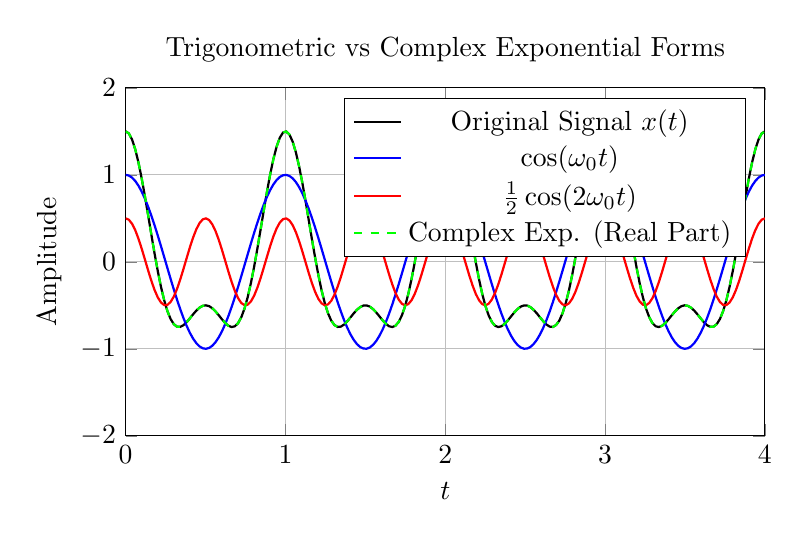
\begin{tikzpicture}
    \begin{axis}[
        width=0.8\textwidth,
        height=6cm,
        xlabel={$t$},
        ylabel={Amplitude},
        title={Trigonometric vs Complex Exponential Forms},
        grid=major,
        xmin=0, xmax=4,
        ymin=-2, ymax=2,
        xtick={0,1,2,3,4},
        ytick={-2,-1,0,1,2},
        legend pos=north east,
    ]
    
    % Original signal
    \addplot[black, thick, domain=0:4, samples=200] {cos(deg(2*pi*x)) + 0.5*cos(deg(4*pi*x))};
    \addlegendentry{Original Signal $x(t)$}
    
    % Trigonometric form components
    \addplot[blue, thick, domain=0:4, samples=200] {cos(deg(2*pi*x))};
    \addlegendentry{$\cos(\omega_0 t)$}
    
    \addplot[red, thick, domain=0:4, samples=200] {0.5*cos(deg(4*pi*x))};
    \addlegendentry{$\frac{1}{2}\cos(2\omega_0 t)$}
    
    % Complex exponential form (real part)
    \addplot[green, thick, dashed, domain=0:4, samples=200] {cos(deg(2*pi*x)) + 0.5*cos(deg(4*pi*x))};
    \addlegendentry{Complex Exp. (Real Part)}
    
    \end{axis}
\end{tikzpicture}
